\begin{figure}[htbp]
\centering
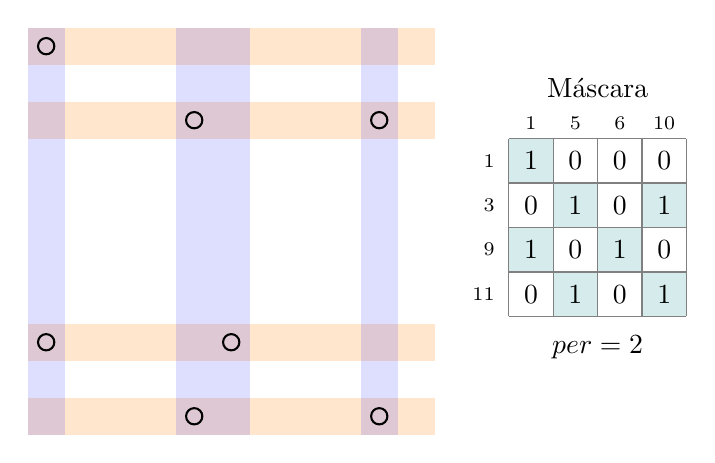
\begin{tikzpicture}[x=.47cm,y=.47cm]
 \bcuadricula{11}
 \foreach \rr in {1,3,9,11}{\fill[orange,opacity=.20] (0,{11-\rr}) rectangle (11,{12-\rr});}
 \foreach \cc in {1,5,6,10}{\fill[blue,opacity=.13] ({\cc-1},0) rectangle (\cc,11);}
 \foreach \rr/\cc in {1/1,3/5,3/10,9/1,9/6,11/5,11/10}{
  \bmarca{11}{\rr}{\cc}
  \draw[black,line width=.75pt] ({\cc-.5},{11.5-\rr}) circle[radius=.22];
 }
 \foreach \rr/\cc in {2/3,4/7,5/9,6/11,7/2,8/4,10/8}{\breina{11}{\rr}{\cc}}
 \begin{scope}[shift={(13,3.2)},scale=1.2]
  \node at (2,5.15) {Máscara};
  \foreach \indice/\original in {1/1,2/5,3/6,4/10}
   {\node[font=\scriptsize] at ({\indice-.5},4.35) {$\original$};}
  \foreach \indice/\original in {1/1,2/3,3/9,4/11}
   {\node[font=\scriptsize,anchor=east] at (-.1,{4.5-\indice}) {$\original$};}
  \foreach \rr/\cc in {1/1,2/2,2/4,3/1,3/3,4/2,4/4}
   {\fill[teal!16] ({\cc-1},{4-\rr}) rectangle (\cc,{5-\rr});}
  \draw[step=1,gray,line width=.45pt] (0,0) grid (4,4);
  \foreach \rr/\valores in {1/{1,0,0,0},2/{0,1,0,1},3/{1,0,1,0},4/{0,1,0,1}}{
   \foreach \valor [count=\cc] in \valores
    {\node at ({\cc-.5},{4.5-\rr}) {$\valor$};}
  }
  \node at (2,-.7) {$\operatorname{per}=2$};
 \end{scope}
\end{tikzpicture}
\caption{Tablero de orden once de la solución $\pi=(1,3,5,7,9,11,2,4,6,8,10)$ después de retirar las
reinas de las filas $1,3,9,11$. Las filas se numeran desde uno de arriba abajo y las columnas desde
uno de izquierda a derecha. Quedan siete reinas, dibujadas con coronas. Las bandas destacan las cuatro
filas vacías y las columnas vacías $1,5,6,10$. Los puntos rodeados señalan las casillas disponibles y
corresponden a los unos de la máscara, que conserva las etiquetas originales. La fila $1$ fuerza la
columna $1$ y entonces la fila $9$ fuerza la $6$. Las filas $3$ y $11$ pueden intercambiar $5$ y $10$,
de donde resulta el permanente $2$. Las diferencias positivas entre filas son $2,6,8,10$ y entre
columnas son $1,4,5,9$. Como los dos conjuntos son disjuntos, los cruces vacíos no comparten
diagonal.}\label{fig:terminal}
\end{figure}
